\documentclass[tikz]{standalone}
\usepackage{pgfplots}
\pgfplotsset{compat=1.15}
\usepackage{mathrsfs}
\usetikzlibrary{arrows,calc}
\usepackage{tkz-euclide}

\pagestyle{empty}

\definecolor{AngleClr}{rgb}{0,0.39215686274509803,0}
\definecolor{ShapeClr}{rgb}{0.6,0.2,0}

\begin{document}

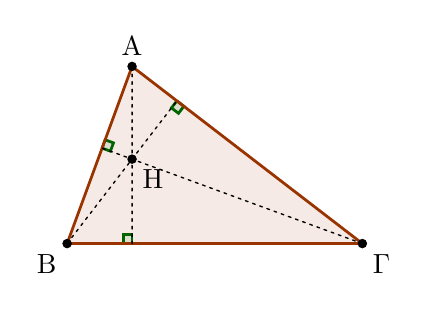
\begin{tikzpicture}[scale=.75]
\tkzSetUpLine[line width=1pt,color=black]
\tkzSetUpPoint[fill=black]

\tkzDefPoints{0/0/B,1.1/3/A,5/0/C}

\tkzDefTriangleCenter[ortho](A,B,C)
\tkzGetPoint{H}

\tkzDefPointBy[projection=onto B--C](H)\tkzGetPoint{HA}
\tkzDefPointBy[projection=onto A--C](H)\tkzGetPoint{HB}
\tkzDefPointBy[projection=onto A--B](H)\tkzGetPoint{HC}

\tkzFillPolygon[fill=ShapeClr,fill opacity=0.1](A,B,C)

\tkzMarkRightAngles[line width=1pt, size=.15,color=AngleClr,fill=AngleClr,fill opacity=0.1](H,HA,B H,HB,C H,HC,A)

\tkzDrawPolygon[color=ShapeClr](A,B,C)


\tkzDrawSegments[line width=0.5pt,color=black,dashed,dash pattern=on 1pt off 1.75pt](A,HA B,HB C,HC)

\tkzDrawPoints[size=3](A,B,C,H)
\tkzLabelPoint[above](A){$\rm A$}
\tkzLabelPoint[below left](B){$\rm B$}
\tkzLabelPoint[below right](C){$\rm \Gamma$}
\tkzLabelPoint[below right](H){$\rm H$}

\end{tikzpicture}
\end{document}
